\section{寻找其他对齐方案比较：从类条件 CORAL 到 LMMD}
\label{sec:alternatives}

\subsection{探索一：把全局协方差匹配改为逐类匹配}

全局协方差同时包含类内变化和类间中心结构；不同类别的域偏移可能在整体统计中相互掩盖。DSAN 通过源域真实类别和目标预测概率建立相关子域，再以 LMMD 对齐其核分布\cite{zhu2021dsan}。本阶段先借用这种软类别分组思路，将统计目标换成逐类协方差，检验能否保留 CORAL 的简洁形式并获得更细的对齐。

在 AlexNet fc8 的 31 维 logits 上，源域权重由 one-hot 标签归一化，目标权重由预测概率归一化：
\begin{equation*}
 p_{jc}=\sg[\operatorname{softmax}(z_j^t)_c],\qquad
 a^s_{ic}=\frac{\mathbf1[y_i^s=c]}{\sum_r\mathbf1[y_r^s=c]},\qquad
 a^t_{jc}=\frac{p_{jc}}{\sum_rp_{rc}}.
\end{equation*}
目标概率停止梯度，但目标特征本身仍参与反向传播。对于被保留的类别，全部目标图像通过其软权重参与统计，top-1 类别用于支持筛选，不是硬分组后的样本截取。加权均值与协方差为
\begin{equation*}
 \mu_d^c=\sum_i a^d_{ic}z_i^d,\qquad
 C_d^c=\frac{\sum_i a^d_{ic}(z_i^d-\mu_d^c)(z_i^d-\mu_d^c)^\top}
 {1-\sum_i(a^d_{ic})^2}.
\end{equation*}
这一有限样本修正在均匀权重下还原样本协方差；特征依赖的软权重不保证总体无偏估计。有效类别集合 $\mathcal V$ 要求源样本数至少 2、目标 top-1 支持至少 2，且目标 $\ESS_c=1/\sum_j(a^t_{jc})^2\ge2$。自定义类条件损失为
\begin{equation*}
 L_C=\frac1{|\mathcal V|}\sum_{c\in\mathcal V}
 \frac{\norm{C_s^c-C_t^c}_F^2}{4D^2},\qquad D=31.
 \label{eq:local}
\end{equation*}
这不是 DSAN 原方法；DSAN 的原始统计目标是核均值嵌入。

\subsection{匹配对照与类条件 CORAL 的结果}

为隔离阶段内的训练差异，重新建立 AlexNet 六组对照，保持相同初始化、batch=128、每轮 6 步、SGD 与预处理，固定训练 50 轮。所有适应组前十轮均使用 $\CE+0.5G$，第 11 轮起切换到表\ref{tab:subdomain}中的适应项；无适应组保留目标前向，使 Dropout 的随机数消耗方式一致。各适应组的前十轮共同指标已在 $10^{-6}$ 容差内核对。

本阶段全局 CORAL 为 53.84\%，与第一部分历史 fc8 的 54.21\% 属于分别归档的运行族。阶段内比较使用重新建立的 53.84\% 对照，不能因表面配置相近而替换分母或拼接曲线。

\begin{table}[H]
 \centering\small
 \caption{AlexNet 子域六组匹配对照。准确率与宏平均类别准确率单位为 \%，均取固定第 50 轮。表中每组均含源域 CE；适应组第 1--10 轮为 $0.5G$。}
 \label{tab:subdomain}
 \begin{tabular}{lcrr}
 \toprule
 配置 & 第 11--50 轮适应项 & 准确率 & 宏平均\\
 \midrule
 \SubdomainRows
 \bottomrule
 \end{tabular}
\end{table}

把全局项完全替换为 $0.5L_C$ 后，准确率为 42.14\%，相对全局 CORAL 为 $-11.70\pp$。保留 $0.25G$ 并增加 $0.25L_C$ 的 mixed 为 49.56\%；相同全局系数、没有局部项的 global\_quarter 为 54.09\%，差值为 $-4.53\pp$。这一额外对照排除了“联合组只是因为全局权重减半”这一单独解释。逐图配对记录中，local 相对 global 修正 14 张，却新增 107 张错误，净差为 $-93$ 张；现象来自分类判定变化，而非结果表的四舍五入。

\subsection{探索二：保留软类别分组，改用 LMMD}

上述结果提出了更具体的问题：逐类划分本身是否不足，协方差目标是否遗漏了分类所需信息？为此追加一组 LMMD，复用五组已完成对照。该组同样经过十轮全局 CORAL 预热，第 11--50 轮改用 $\CE+0.5M$。模型、轮数、采样与初始化保持匹配，改变的是局部统计目标及其作者支持规则；它不是完整 DSAN 架构复现。

LMMD 使用相同的源域 one-hot 与目标软概率权重，在再生核 Hilbert 空间中匹配类别条件均值\cite{zhu2021dsan}：
\begin{equation}
\begin{aligned}
 M&=\frac1{|\mathcal U|}\sum_{c\in\mathcal U}
 \left\|\sum_i a^s_{ic}\phi(z_i^s)-\sum_j a^t_{jc}\phi(z_j^t)\right\|_{\mathcal H}^2,\\
 M_c&=\sum_{i,i'}a^s_{ic}a^s_{i'c}k(z_i^s,z_{i'}^s)
 +\sum_{j,j'}a^t_{jc}a^t_{j'c}k(z_j^t,z_{j'}^t)
 -2\sum_{i,j}a^s_{ic}a^t_{jc}k(z_i^s,z_j^t).
\end{aligned}
\label{eq:lmmd}
\end{equation}
作者代码以源真实类与目标 top-1 类的交集为 $\mathcal U$，每域出现一个支持样本即可，不设 ESS 门槛；域内求和保留对角线，使用 V-statistic。核为五个 RBF 核之和，带宽取拼接批次非对角平方距离的均值并停止梯度，具体公式见附录。该约定依照归档作者实现\cite{dsancode}，并非将论文的带宽文字描述直接当作代码行为。

\begin{figure}[H]
 \centering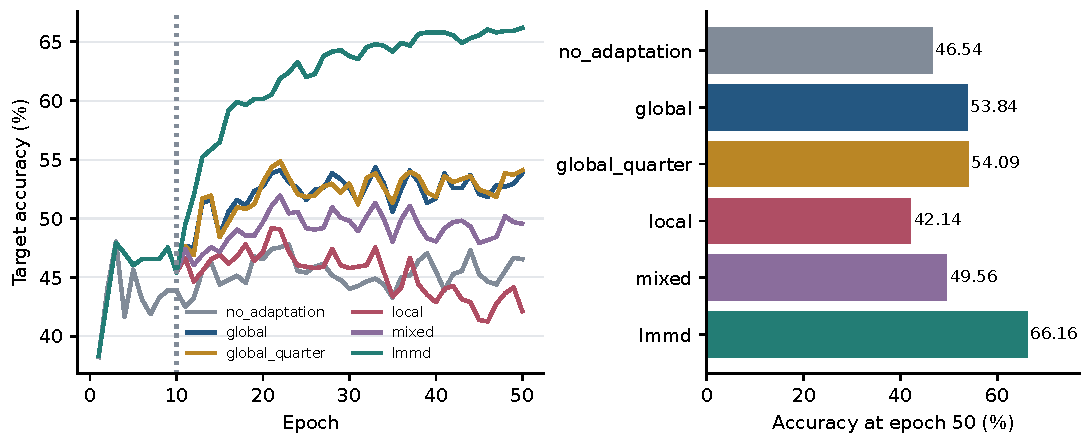
\includegraphics[width=\linewidth]{subdomain.pdf}
 \caption{AlexNet 六组训练与固定轮结果。虚线为十轮预热结束；LMMD 第 50 轮达到 66.16\%。全部适应组共享预热协议，阶段内全局对照为 53.84\%。}
 \label{fig:subdomain}
\end{figure}

LMMD 的第 50 轮准确率为 66.16\%，相对 global 为 $+12.33\pp$，相对 local 为 $+24.03\pp$。相对 global，LMMD 修正 119 张而新增 21 张错误，净增加 98 张正确预测；宏平均类别准确率同为 66.16\%。图\ref{fig:subdomain}表明，这一收益出现在预热后训练过程中。匹配对照支持继续研究“类别软分组与核分布匹配”的组合，而不是直接放弃类别条件对齐。

\subsection{结果反思：更小的协方差距离为何没有更好的分类？}

对六组固定最终模型进行全域 logits 诊断，关闭 Dropout，以真实类别计算协方差距离与中心方向；目标真值在此用于训练后的解释。表\ref{tab:geometry}及图\ref{fig:geometry}选择 global、local、LMMD 三组展示。

\begin{table}[H]
 \centering\small
 \caption{固定第 50 轮的事后几何诊断，使用原始 logits。$D_C$ 为真实类协方差距离，$D_{\rm dir}$ 为真实类中心余弦距离，$Q$ 为目标软类别权重纯度。距离对类别等权平均，定义见附录。}
 \label{tab:geometry}
 \begin{tabular}{lrrrr}
 \toprule
 配置 & $D_C$ & $D_{\rm dir}$ & 目标平均范数 & $Q$\\
 \midrule
 \GeometryRows
 \bottomrule
 \end{tabular}
\end{table}

\begin{figure}[H]
 \centering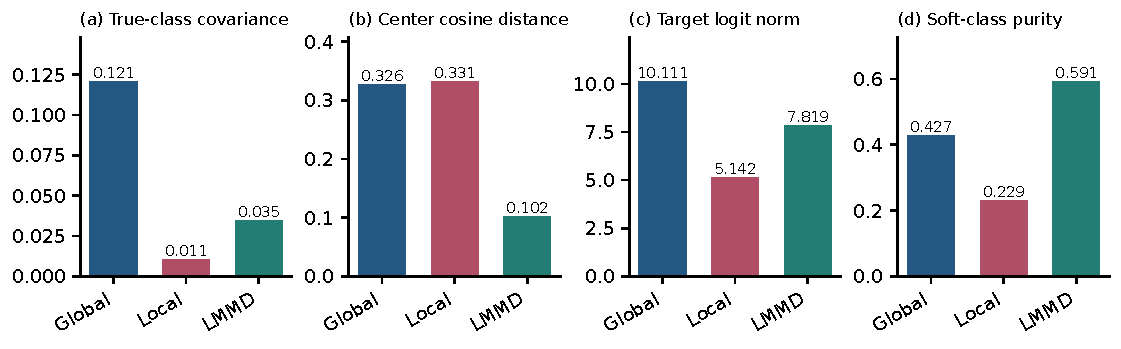
\includegraphics[width=\linewidth]{geometry.pdf}
 \caption{协方差、类别中心、幅度与软分组的联合诊断。local 的协方差距离最小；LMMD 的中心方向距离更小、软权重纯度更高。各面板独立标度，指标排序不等同于因果贡献。}
 \label{fig:geometry}
\end{figure}

\textbf{第一，类内协方差不直接约束类别中心。}固定类别权重时，各域独立平移不改变其协方差：
\begin{equation*}
 C_a(Z+\mathbf1v^\top)=C_a(Z).
\end{equation*}
即使源目标同类中心不同，类条件 CORAL 也可为零。local 的 $D_C$ 比 global 小约 91.3\%，中心方向距离却由 0.326 变为 0.331。LMMD 的 $D_C$ 为 0.03481，大于 local 的 0.01053，但中心方向距离为 0.102，分类准确率也更高。由此可见，减小类内波动差异与改善类别位置是不同目标。

\textbf{第二，绝对二阶距离具有尺度捷径。}固定权重、令两域表示共同缩放为 $sZ$，有 $L_C(sZ_s,sZ_t)=s^4L_C(Z_s,Z_t)$。local 的目标平均范数从 global 的 10.11 变为 5.14，目标协方差迹从 97.93 变为 24.27，与尺度收缩相符。不过，去除逐图共同 logit 偏移后的协方差形状距离也有所改善，说明二阶匹配变化不全由缩放解释；local 的目标有效秩为 25.19，且仍预测到全部 31 类，现有证据不支持将其称为低秩或单点坍塌。

进一步去除不影响 softmax 的共同 logit 偏移后，local 的类中心方向距离仍为 0.331，其归一化分类 margin 中位数为 $-0.086$，global 为 0.033；二者不会因共同正缩放而改变。目标类间协方差迹分别为 9.17 与 45.93，LMMD 为 39.45。较小的类内差异可以伴随类别间结构收缩，这比单看原始损失更贴近本次分类现象。

\textbf{第三，软权重的覆盖与纯度需要分开。}local 的软分组纯度为 0.229，global 为 0.427，LMMD 为 0.591；其全域平均 ESS 却从 global 的 60.30 增至 177.03。更大的 ESS 表示权重较分散，不表示集中于更多正确同类图像。被保留类别内，若概率对不同图像缺少区分，归一化软权重便接近均匀，其统计量会趋近全域统计而失去清晰类别含义。软分组混杂与局部约束可能形成相互强化的过程，这是与诊断一致、仍需干预实验检验的解释。

\textbf{第四，LMMD 改变了统计信息与类别利用方式。}线性核下式\eqref{eq:lmmd}就是类别中心差平方；RBF 核进一步感知非线性分布结构。固定带宽的高斯核在总体层面是特征核，MMD 为零可以识别分布相等\cite{gretton2012kernel}，但这一性质不等价于有限批次、预测软分组下的零分类误差。作者每批重估带宽时，在带宽下限未触发、类别权重固定的条件下，共同缩放不会改变核值；这一前向性质使 LMMD 的数值不因两域一起缩小而自动改善。带宽停止梯度意味着不能进一步把它解释为训练梯度的尺度不变性。

训练第 11--50 轮，local 按 CORAL 规则平均保留 21.92 类；LMMD 按作者规则为 29.37 类，同一 LMMD 运行按 CORAL 规则监测为 24.89 类。LMMD 不需要逐类协方差的双样本支持，因而可以利用更多共享类。同时，其加权损失量级也不同：第 50 轮为 0.41433，global 的加权 CORAL 为 0.04126。该比较没有匹配的适应梯度记录，不能把损失值之比当作梯度强度之比，也不能把收益全部归因于核函数。

\subsection{探索三：采用 ResNet-50 的 DSAN 作者代码配方}

AlexNet 的匹配实验给出了继续采用 LMMD 的依据。随后使用 ResNet-50 V2 与 256 维 bottleneck，按 DSAN 作者代码口径开展一组独立实验。模型为 $2048\to256\to31$，新增两层 Linear 之间不加 ReLU、Dropout 或 BN，对齐 256 维 bottleneck。该实验采用 batch=32、源域驱动的 87 步/轮、目标批次循环复用，不使用 CORAL 预热。

学习率按作者衰减，适应权重按预定训练进度渐增至 0.5；这与第二部分根据梯度反馈学习的自适应 $\lambda$ 是两种不同机制。训练输入采用 Resize(256)、随机裁剪至 224、随机水平翻转和 ToTensor，不增加 Normalize；评估为 Resize(224) 与 ToTensor。保留共享 BN，预算为 200 轮，每轮用目标准确率更新最佳记录，30 轮无严格提高即停止。

\begin{figure}[H]
 \centering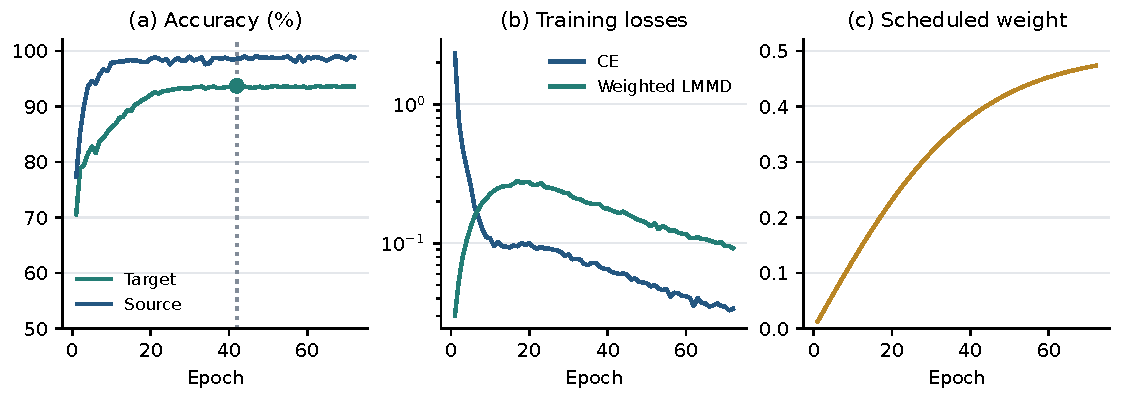
\includegraphics[width=\linewidth]{resnet_lmmd.pdf}
 \caption{ResNet-50 V2 的 LMMD 独立实验。第 42 轮最佳为 93.71\%，第 72 轮停止为 93.58\%；目标真值参与选轮和停止。右图为预设权重调度，不是梯度范数控制。}
 \label{fig:resnetlmmd}
\end{figure}

该组完成 72 轮、6,264 步，第 42 轮最佳为 93.71\%，第 72 轮停止为 93.58\%（图\ref{fig:resnetlmmd}）。DSAN 原论文报告 A$\to$W 为 $93.6\pm0.2\%$，对应三次随机实验的均值与标准误\cite{zhu2021dsan}；本地单次结果与其处于相近数值区间，但预训练、实现及选择条件不同，不能据此声称统计复现或超越。

与第三部分相比，本组同时改变了 bottleneck、增强、归一化、每轮步数、学习率、权重调度和结果选择方式。因而 93.71\% 与旧 CORAL 的 81.76\% 不构成匹配的损失替换对照，两者差值不能作为 LMMD 的独立收益。它说明的是这套完整配方的本地表现；LMMD 的阶段内直接比较依据仍是表\ref{tab:subdomain}。

\subsection{阶段结论与反思}

本阶段最清晰的结果是：\textbf{在匹配 AlexNet/fc8 与预热配置下，LMMD 达到 66.16\%，自定义类条件 CORAL 为 42.14\%。}类条件 CORAL 已改善真实类二阶统计，却没有改善分类；问题不能简单归为损失没有优化成功。中心位置、尺度以及软分组质量的诊断，将反思从“是否继续增加约束”推进到“统计目标是否约束了任务需要的信息”。

后续检验应围绕这些解释设置干预：统一两种局部损失的支持集合，以训练内梯度统计校准强度，再比较软类别均值匹配、协方差匹配及其联合；对软标签可靠性进行独立干预，观察纯度、中心方向与分类是否共同变化。LMMD 的优势也需要在这些因素固定后判断。由此保留 LMMD 作为继续探索的工作参照，并把类别几何与优化强度分开验证，而不是将任一事后诊断升级为普遍的性能代理。
